\chapter{Methods}
In this chapter the basics of the Lattice Boltzmann Method are explained.
This includes the Probability Density Function, Boltzmann Transport Equation and more.


\section{Probability Density Function}
Imagine a 2d grid-like space with discrete positions, where each positions is called a lattice point.
This space contains many particles, each flowing around in different directions but always being confined to a specific lattice point.
For this space it's possible to determine the probabilistic density of a specific lattice point.
The Probabilistic Density Function does this given the points \(\mathbf r\) and velocities \(\mathbf v\)
\[f(\mathbf r ,\mathbf v,t)\].


\section{Lattice Boltzmann Transport Equation (BTE)}
Remember the 2d gridlike space from before.
It is important to also define the movement of each particle.
This movement is given by the Boltzmann Transport Equation which consists of the two parts streaming and collision.
Both are explained in the following subsections.

\subsection{Streaming}

\begin{figure}[h!]
    \begin{center}
        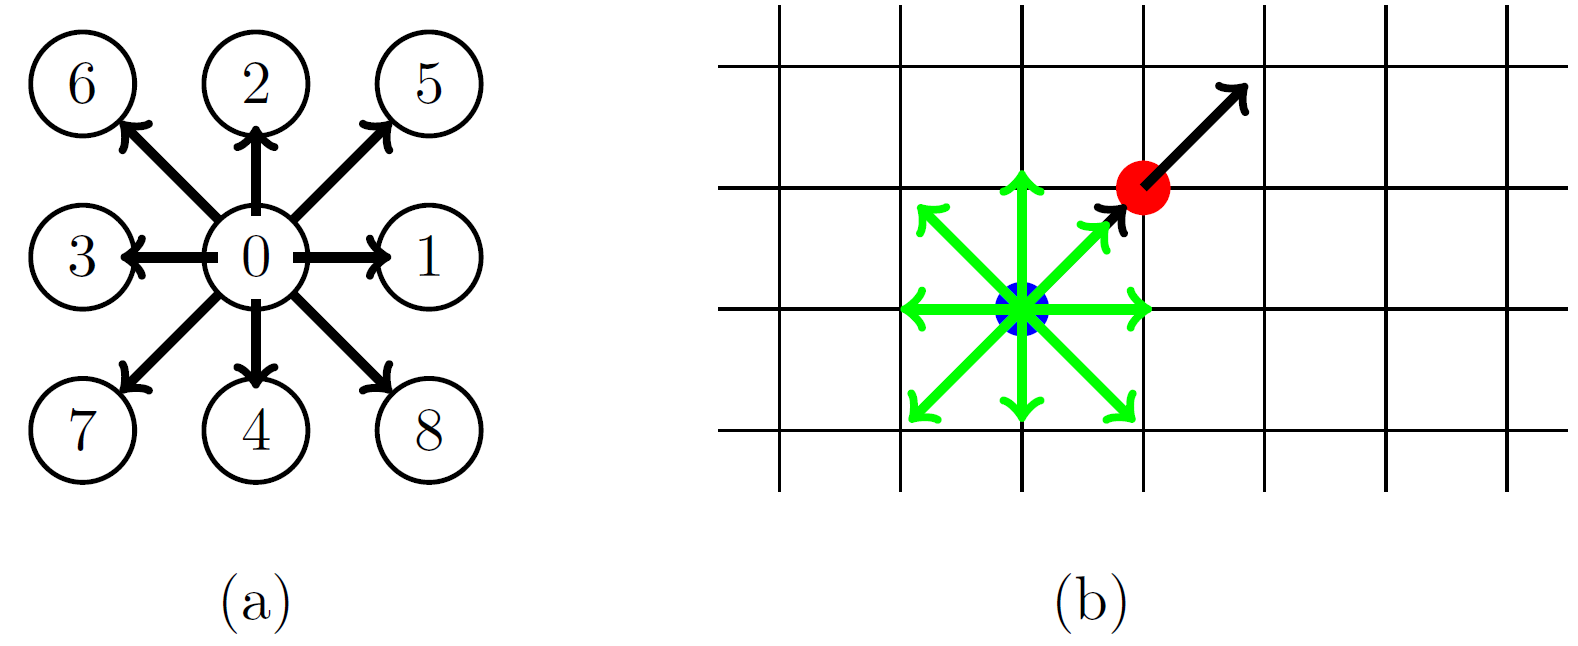
\includegraphics[width=10cm]{logos/Gitter_LBM.png}
        \caption[Visualization of the underlying grid including labled directions.]{
            Visualization of the underlying grid including labled directions. \\
            (a) directions with given labels \\
            (b) streaming example of one particle
        }
        \label{fig:bte}
    \end{center}
\end{figure}

During the streaming, each particle moves in one of a set of predefined directions.
These particles can be further abstracted to densities, moving in specific directions.
The directions are given by the underlying grid and visualized in \ref{fig:bte}.
Each direction has a number in the interval [0, 8], e.g.\ direction 0 symbolizes \textit{not moving} and density with the direction 1 \textit{move to the right}.
To allow moving further than to the closest neighbour, this streaming step is applied at each timestep (this is shown in part b) of \ref{fig:bte}).
Multiple streaming steps therefore allow the fluid to move freely in the space.
\begin{equation}
    \frac{\partial f\left(\mathbf{r},\mathbf{v},t\right)}{\partial t}+\mathbf{v}\nabla_{\mathbf{r}} f\left(\mathbf{r},\mathbf{v},t\right)
    +\mathbf{a}\nabla_{\mathbf{v}} f\left(\mathbf{r},\mathbf{v},t\right)=C(f).
\end{equation}

\subsection{Collision}
The streaming allows particles to move through space, however it is missing the interaction between the particles.
This interaction is resembled by collision.
Collision is best described as an exchange of energy and momentum between two particles.
In the simulation a truly instant exchange is not possible as computations happen iteratively.
However it is possible to apply collision in the same timestep as the streaming.
This results in a simultaneous exchange in the context of the simulation.
Another benefit of this approach is the possibility to determine the equilibrium function of \(f^{eq}\left(\mathbf{r},\mathbf{v},t\right)\) at each timestep.
With \(f^{eq}\) the calculation of the collision results in

\begin{equation}
    \frac{d}{dt} f\left(\mathbf{r},\mathbf{v},t\right) = -\frac{ f\left(\mathbf{r},\mathbf{v},t\right)- f^{eq}\left(\mathbf{r},\mathbf{v},t\right)}{\tau}
    \cdot
    \label{eq:bgk}\tag{1}
\end{equation}

\subsection{Equilibirum Function}
To apply collsion an equilibirum function needs to be determined.
This part explains how to do that.
To determine how to calculate it, first a look at the equation and the missing parts is needed.
The formula of the equilibrium function is given by
\begin{equation}
    f_i^{eq}(\rho(\mathbf{r}),\mathbf{u}(\mathbf{r}))=w_i\rho(\mathbf{r})
    \left[1
    +3\mathbf{c}_i\cdot\mathbf{u}(\mathbf{r})
    +\frac{9}{2}\left(\mathbf{c}_i\cdot\mathbf{u}(\mathbf{r})\right)^2
    -\frac{3}{2}|\mathbf{u}(\mathbf{r})|^2
    \right]
    \cdot
    \label{eq:feq}\tag{5}
\end{equation}

Having a look at \ref{eq:feq}, the density \(\rho(\mathbf{r})\), velocity \(\mathbf{u}(\mathbf{r})\) and \(w_i\)  still needs to be determined.
Each of them can be determined given the next formulas, where \(w_i\) is defined for a D2D9 lattice:

\begin{equation}
    f_i(\mathbf{r}+\Delta t\mathbf{c}_i,t+\Delta t)
    =f_i(\mathbf{r},t)+\omega\left(f_i^{eq}(\mathbf{r},t)-f_i(\mathbf{r},t)\right)
    \label{eq:DBTE}\tag{2}
\end{equation}

\begin{equation}
    \label{eq:rho}\tag{3}
    \rho(\mathbf{r})=\sum_i f_i
\end{equation}

\begin{equation}
    \label{eq:u}\tag{4}
    \mathbf{u}(\mathbf{r})=
    \frac{1}{\rho(\mathbf{r})}\sum_i \mathbf{c}_i f_i(\mathbf{r})
\end{equation}



\begin{equation}
    w_i = \left(\dfrac{4}{9},
    \dfrac{1}{9}, \dfrac{1}{9}, \dfrac{1}{9}, \dfrac{1}{9},
    \dfrac{1}{36}, \dfrac{1}{36}, \dfrac{1}{36}, \dfrac{1}{36}\right)
\end{equation}
